At this point, we proceed with the evaluation of the results showed in the previous section. As the concept of recommendation changes from a context to another and it depends also on the developer's skills (maybe a more expert user finds a certain recommendation less useful rather than a not expert user), we look for an evaluation framework that evaluates the results without bias related to this aspect. To do this, we choose Rascal tool to parse the AST of the developer's file and the API recommendations obtained combining Simian and CLAMS results. From Rascal, we obtain a list of method declarations and the related invocations for each file and compare them in order to calculate four metrics: precision, recall, success rate and F measure. These metrics are very useful because they allow to analyze the results at more abstract level, going beyond the code cloning activity. In facts, as we said in the related section, Simian not perform this kind of comparison because it is a textual code cloner and looks only for duplicated lines of code. The main structure of the validation framework is depicted in Figure 5. Moreover, we compare the proposed approach with PAM, the probabilistic tool already analyzed in term of results, computational time and also by applying the same metrics on the method invocations. Next sections explains in details each component of this system, especially how to run Rascal and how the metrics have been calculated and how covert the PAM format in order to perform the comparison in the right manner.




\begin{figure}[H]
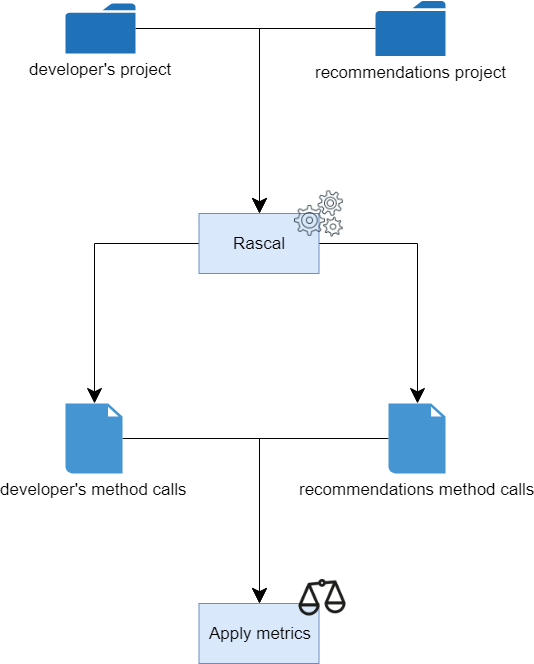
\includegraphics[width=14cm,height=14cm,keepaspectratio]{images/rascal.png}
\centering
 \caption{Validation framework}
 \label{fig:cmd}
\end{figure}

\subsection{Research questions}
The research question are the following: \\

\textbf{RQ$_1$} \textit{ Is it the approach able to provide consistent recommendation?}
This research question measures the quality of the recommendations provided by comparing the context, represented by the round truth part, and the retrieved patterns by the proposed approach. We analyze possible situation in which there are some false positive situations by computing the metrics mentioned before and report the results in order to make an evaluation at the level of method invocations.\\
\textbf{RQ$_2$} \textit{Are the final results good enough compared with PAM?} In order to validate the proposed approach, we perform a comparison with PAM, the tool presented in the existing approach section and compute the metrics also on it. We provide a comparison between the two approaches by looking the average metrics values. PAM produces a list of method invocations, so to do in a better way the comparison we used Rascal to transform the recommendations provided by our approach in method invocations. It is necessary to computes the metrics\\

\textbf{RQ$_3$} \textit{What are the timing performances of the proposed approach?} With this research question, we measure the time computation for a single recommendation. We take into account also the time needed to write the output file with the recommended snippet of code and compare it with PAM. We added the time comparison because it is crucial factor in a recommendation system. We measure the time in seconds.\\

\subsection{Study methodologies}
To validate and apply the metrics, we simulate the typical scenario in which the developer is working on a project. To do this, we select randomly a fragment of code coming from the client file using Java Parser as described before. We obtain in this way our context, that is only a small part of the original file and perform our approach on it. To apply metrics, however, we need a transformation from the snippet of code to method invocations, that is a more comparable format. To do this, we use Rascal \cite{utor.rascal-mpl.org/_last_nodate}, a language for meta programming and it is able to create programs that read, analyse, transform, generate and/or visualize other programs. The range of programs to which meta-programming can be applied is large: from programs in standard languages like C and Java to domain-specific languages for describing high-level system models or applications in specialized area. In some cases, even test results or performance data are used as input for meta-programs. We look also to the kinds of meta programs that can be analyzed by Rascal like reverse engineer and statically analyse of a big software system before visualizing the results. The principal aim of Rascal is to provide a reusable set of primitives to build and manipulate program representations. The point is not to be or provide a unified representation of programs to let generic algorithms operate on.  
We can look also at Rascal as an engineering tool for programmers that need to construct meta programs because it allows running, inspecting, debugging, tracing, profiling, etc. just as normal programs do. The main advantages are:
\begin{itemize}
\item The syntax is very easy to learn and is used even for model and represent sophisticated concepts;
\item Sophisticated built-in data types provide standard solutions for many meta-programming problems;
\item Safety is achieved by finding most errors before the program is executed, so the debug phase is reduced;
\item Local type inference makes local variable declarations redundant;
\item Pattern matching can be used to analyze all complex data structures;
\item Syntax definitions make it possible to define new and existing languages for specific purposes;
\item Traversing the data structures is doing in an effective way and it is possible to extract information from them or to synthesize results;
\item Templates enable easy code generation;
\item The integration in Eclipse simplify the usage and the iteration with all Rascal features.
\end{itemize}
Moreover, Rascal implements the so called EASY(Extract-Analyze-SYnthesize) paradigm, used in the meta programming domain.  ny meta-programming problems follow a fixed pattern. Starting with some input system (a black box that we usually call system-of-interest), first relevant information is extracted from it and stored in an internal representation. This internal representation is then analyzed and used to synthesize results. If the synthesis indicates this, these steps can be repeated over and over again. Figure 6 represents the EASY paradigm that is quite common in the meta programming domain.

\begin{figure}[H]
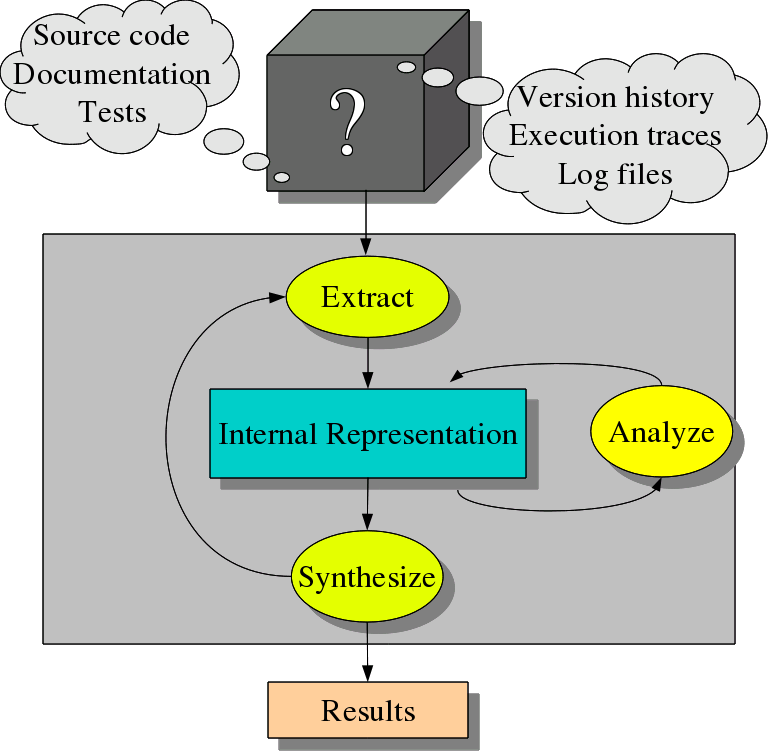
\includegraphics[width=10cm,height=12cm,keepaspectratio]{images/EASY.png}
\centering
  \caption{The EASY paradigm used by Rascal}
  \label{fig:cmd}
\end{figure}

For our purposes, we use Rascal to parse AST of an entire project and retrieves all necessary information from it, such as class names, packages, methods and variables.
To do this, however, it needs a runnable project and the classpath file in which all dependencies are specified. In our scenario, the only required dependency is the jar file for the library. As the evaluation takes places among method invocations, we are forced to create this structure for the developer's file and the patterns that represents our recommendations. The structure is represented in Figure 7, in which we have:
\begin{itemize}
\item src folder: it contains the Java file with the source code;
\item lib folder: it contains the jar files that represent the libraries used in the project;
\item classpath file: it contains the dependencies for the project.
\end{itemize}

\begin{figure}[H]
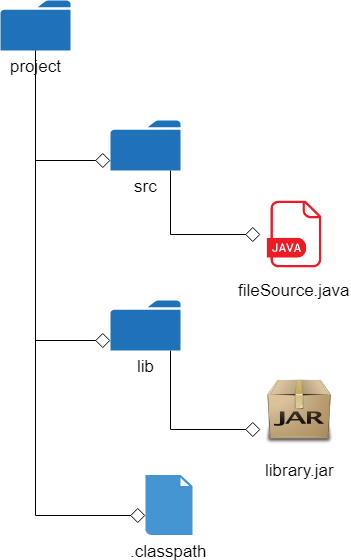
\includegraphics[width=12cm,height=12cm,keepaspectratio]{images/Folders.png}
\centering
  \caption{Folder structure for Rascal}
  \label{fig:cmd}
\end{figure}

Where the file in the src folder represents the developer's file in one project and the recommendations in the second one. These two projects will be the input of Rascal. All the structure is built in the evaluation subpackage as mentioned before. In particular, we functions that takes as input the library name and gives the correct classpath file to have the structure mentioned before. Moreover, we have a function that build the class in the correct way putting together the CLAMS patterns in a single class (for each of them, the function creates a method) where at the beginning the same import of the ground truth are inserted. For the patterns, we take as import the same contained in the namespaces file included in the original CLAMS dataset, in order to have all possible method invocations. Also for the ground truth we make a similar structure, by putting the considered method in a Java class in the Rascal structure. We make this task for the ten client projects for each considered library twice, because we want to analyze also the pattern in form of snippet of code extracted by the proposed approach. For the ground truth fragments of code, we put all imports used in the original client file; for the mined patterns, we encode in the built files all the imports that belong to the CLAMS namespace file. This task is necessary because we don't know at the beginning what are all the possible recommendations and so the possible method invocations. This approach cannot bring any bias because Rascal retrieves only the method invocations with the corresponding import. Here below we have an example file created for Rascal:
\begin{lstlisting}
import twitter4j.Query;
import twitter4j.Tweet;
import twitter4j.Twitter;
import twitter4j.TwitterFactory;
public class Twitter4jSample{
public void ground() {
    List<MyTweet> tweets = new ArrayList<MyTweet>();
    try {
        // get some tweets about java
        Twitter twitter4j = new TwitterFactory().getInstance();
        for (int i = 0; i < 3; i++) {
            Query q = new Query("java");
            q.setRpp(100);
            for (Tweet tw : twitter4j.search(q).getTweets()) {
                MyTweet myTw = new MyTweet(tw.getId(), tw.getFromUser());
                myTw.setText(tw.getText());
                myTw.setCreatedAt(tw.getCreatedAt());
                myTw.setFromUserId(tw.getFromUserId());
                tweets.add(myTw);
            }
            Thread.sleep(1000);
        }
    } catch (Exception ex) {
        logger.error("Error while grabbing tweets from twitter!", ex);
    }
    return tweets;
}
}
\end{lstlisting}
In particular, we have added the fragment of code pick up from the developer's client file and put it a method called ground, plus the required imports for the snippet.
Once we setup this structure in this way, Rascal is able to parse the AST and retrieve the list of method invocations used to validate the approach.
Rascal is launched using Eclipse RCP-RAP as platform and, for this reason, we must use it as standalone to produce the list of method invocations starting from the output file of Simian and CLAMS. The main component of Rascal is module in which we define the function used for our purpose. In particular, the proper function is called on the project's folder and gives as output a file that contains the method invocations. As we said, it is possible by creating the AST and takes from it method declaration and invocations. Here below, we can see an example of a set of method invocations, related to the previous MQTT ground truth example and the second one that contains the method invocations of the mined patterns by Simian related to the MQTT library:\\
Method invocations of the ground truth

\begin{lstlisting}
MqttSample/ground()#org/eclipse/paho/client/mqttv3/MqttMessage/MqttMessage(byte[])
MqttSample/ground()#org/eclipse/paho/client/mqttv3/MqttMessage/setQos(int)
MqttSample/ground()#java/lang/System/currentTimeMillis()
\end{lstlisting}

\vspace{5mm}
\noindent
Method invocation of the mined patterns
\begin{lstlisting}
MqttSample/pattern56()#org/eclipse/paho/client/mqttv3/MqttMessage/MqttMessage(byte[])
MqttSample/pattern56()#org/eclipse/paho/client/mqttv3/MqttClient/MqttClient
(java.lang.String,java.lang.String)
MqttSample/pattern56()#org/eclipse/paho/client/mqttv3/MqttClient/disconnect()
MqttSample/pattern56()#org/eclipse/paho/client/mqttv3/MqttMessage/setQos(int)
MqttSample/pattern56()#org/eclipse/paho/client/mqttv3/MqttClient/publish
(java.lang.String,org.eclipse.paho.client.mqttv3.MqttMessage)
MqttSample/pattern56()#org/eclipse/paho/client/mqttv3/MqttClient/connect()
MqttSample/pattern56()#java/lang/String/getBytes()
MqttSample/pattern56()#org/eclipse/paho/client/mqttv3/MqttClient/setCallback
(org.eclipse.paho.client.mqttv3.MqttCallback)
MqttSample/pattern59()#org/eclipse/paho/client/mqttv3/MqttMessage/MqttMessage(byte[])
MqttSample/pattern59()#org/eclipse/paho/client/mqttv3/MqttMessage/setQos(int)
MqttSample/pattern59()#org/eclipse/paho/client/mqttv3/IMqttToken/waitForCompletion()
MqttSample/pattern59()#java/lang/System/currentTimeMillis()
MqttSample/pattern27()#org/eclipse/paho/client/mqttv3/MqttMessage/MqttMessage(byte[])
MqttSample/pattern27()#org/eclipse/paho/client/mqttv3/MqttMessage/setQos(int)
MqttSample/pattern27()#org/eclipse/paho/client/mqttv3/MqttMessage/setRetained(boolean)

\end{lstlisting}
As it is, these files are not so suitable for an immediate comparison. However, we can apply metrics used in the statistic and information retrieval domains in order to evaluate the Simian approach going beyond the lexical code cloning activity, trying to evaluate the results from a different point of view.
We also select the code fragments that compose our ground truth, trying to coverage the most important objects and methods for each library. To do this, we compose different scenarios, one in which Simian analyzes the first lines of a certain method, another in which we pick the last method and so on. The aim is to cover all the possible features that a certain library offers. For example, for Twitter4j library, we select snippets of code that have both methods for user authentication procedure and methods and procedure to publish a tweet.
\subsection{Dataset}
First of all, we show the list of libraries that the proposed approach supports. They are the same of CLAMS, as they are already tested and most popular in the Java project context. We select 5 libraries among the CLAMS original dataset and they are showed in Table 7. In the table we show also the number of recommended pattern provided by CLAMS, that measure the level of support offered by it. For each library, we select 10 files among these files in order to keep the same context and to perform average values for the metrics. From this, we build our dataset that contains 50 files. Notice that each file represent the developer's file that we have seen in the proposed approach figure and we extract from them the ground truth part. For each of them, we run the proposed approach and evaluate the results through the metrics and the comparison with PAM.
\begin{table}[H]
  \caption{ Libraries supported by Simian and CLAMS }
  \label{Table:7}
 \begin{center}

\begin{tabular}{|c|c|c|}

\hline
 \textbf{Library} & \textbf{No. of patterns}  \\
\hline
 twitter4j &  107   \\
\hline
drools & 309 \\
\hline
camel & 152  \\
\hline 
wicket & 717  \\
\hline
restlet-framework & 182  \\
\hline
\end{tabular}
\end{center}
\end{table} 
Here we provide also a brief description of the our golden set:
\begin{itemize}
\item twitter4j: it is used for integrate the Twitter services in Java environment;
\item drools: it is a Business Rules Management System(BRMS) that helps to define the internal rule for the language;
\item camel: it defines mediation rules and routing for specific domain languages;
\item wicket: it is a component based web framework;
\item restlet framework: it helps to build web APIs following the REST architecture. 
\end{itemize}




\subsection{Metrics}
Once we have the two lists of method invocations, we can define metrics to do the evaluation. They are precision, recall,  f measure and success rate showed below:\\


\begingroup

\fontsize{15pt}{24pt}\selectfont
\noindent
$ Precision =  \frac{corr}{all_{rec}}\\  
\\
Recall  = \frac{corr}{all_{gt}} \\  
\\
F\,Measure =\frac{2*precision*recall}{recall+precision}\\
$

\begin{equation}
 \text{Success rate} =
    \begin{cases}
      1 & \text{if at least one method of the ground truth }\\
      & \text{belongs to the recommended pattern invocation}\\      
      0 & \text{otherwise}
    \end{cases}       
\end{equation}

\endgroup



Where the $corr$ is the number of correct API method invocations by the approach related to the context, $all_{rec}$ is the number of method invocations in the recommendations and $all_{gt}$ are all method invocations of the ground truth part, extracted from the initial files. With the first metric, we want to measure the precision of the recommendations related to the context considering all the patterns and so all the method invocations related to them. The recall, instead, point out the rate related to the ground truth part, that is more restricted than the original file and so, in this case, Simian gives as out put less method invocations but more focused on the context in which we are. The F measure considers both precision and recall in order to give an average value on the accuracy of the approach. The classical index considers the harmonic mean between precision and recall. Finally, the success rate is a binary value that is equal to 1 if at least one method in the ground truth is found in the recommendation, 0 otherwise. In the table, we measure this index for all ten clients and so we give a rate that represents an average success rate.
All the rates goes from 0 to 1 and represent the accuracy of the approach. These number is affected also by the number of patterns extracted by CLAMS. The metrics are computed by using Eclipse, and in particular, once we have the files coming from the Rascal computation, described in the previous section, the function applyMetrics calculates all the metrics specified above.

\subsection{Results}

These metrics work on the method declarations and invocations, so for each mined patterns by the approach we can have a taste of the results. In particular, we go further with respect to the code cloning analysis, that looking for only the lexical differences among the lines of code. Reversely, we are able to adding some postprocessing phase on the results and we can do more accurate comparison with this evaluation framework. 
 We also make a comparison between the proposed approach and an existing API recommendations already presented in the related work section, PAM. The metrics are useful to evaluate the accuracy of Simian applied to CLAMS but we decide to improve the validation framework adding an existing and validated approach. As we said, PAM uses probabilistic techniques in order to retrieve the most probable method invocation starting from file in ARFF format, that contains method invocations and declarations. We can compare the result of PAM with the proposed approach considering the top rank method invocations retrieved by CLAMS (notice that the ranking is based on the duplicated lines of code founded between the original code and the patterns). As the format of our recommendation strongly differs from the PAM format, we have to used once again Rascal to extract the method invocations that represent the API recommendations of the ground truth. What is different is the ranking method to order the list of method invocations. The real issue is to bring the code snippet format towards the PAM format to make a fair comparison. To do this, first of all we have to the same inputs for the tools involved in the comparison. In the case of CLAMS, we can keep trace of the context with the ARFF, that contains the method caller and calls for the library as we described in the proper section, and the clients file, that represent the real implementation in Java. On the other hand, PAM takes as input only the ARFF file without any clients files for the context; so, it is necessary to represent the context in we are in order to reduce bias in the analysis. We can do this by converting the clients files (that are Java source code) in the ARFF format and combine the original files with this new one. We can reuse Rascal in the same way seen in the metrics evaluation, by extracting the method invocation from the clients file. After this phase, we have to transform the method invocations into ARFF format. We can do this with a Python script that converts the file in the right format and combine the original ARFF file with the clients invocations in only one file, that represent the developer's context. In this way, PAM is able to keep trace of the context and produce as final output the list of API function call. After we run PAM, it produces the results in the format already specified in the proper section, in form of method invocations and the corresponding probability. However, as the ground truth are usually only a fragment of the original developer's file, the invocations have small probabilistic impact because the original ARFF file for each libraries have more than 2,000 lines. So, in order to apply metrics for the comparison, we are forced to split the PAM result files and select the section in which we find proper invocations. The figure explains all phases needed for obtain the same format used in the comparison:
 

\begin{figure}[H]
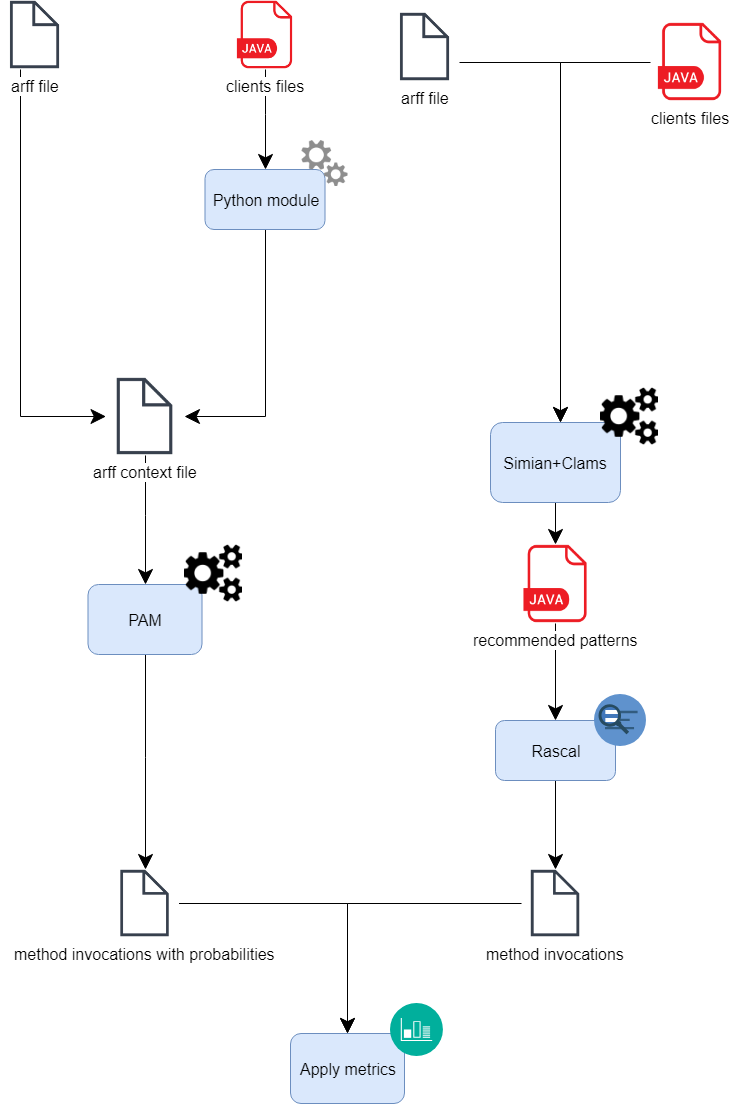
\includegraphics[width=16cm,height=16cm,keepaspectratio]{images/PAM.png}
\centering
  \caption{Process for PAM comparison}
  \label{fig:cmd}
\end{figure}
 At the end of the process, we have the list of invocations ranked by probabilities from PAM and the list of invocations extracted by Rascal. As we have the same format, we can apply the metrics in the same way described before. The two tables offers a comparison between the proposed approach and PAM: 

\begin{table}[H]
  \caption{ Average values for the proposed approach }
  \label{Table:8}
 \begin{center}
\begin{tabular}{|c|c|c|c|c|}

\hline
 \textbf{Library} & \textbf{precision}  & \textbf{recall} & \textbf{success rate} & \textbf{F-measure} \\ 
\hline
 twitter4j &  0,506235119 & 0,74285538 &  0,9 & 0,545789625 \\
\hline
drools & 0,22455129 &   0,344444445 & 0,7 & 0,215914793\\
\hline
camel & 0,430785693  & 0,598096273 & 1 & 0,448844577 \\
\hline 
wicket & 0,104704642 & 0,23564139 & 0,6 & 0,152584271 \\
\hline
restlet-framework &  0,292169883 &  0,539874547 & 0,7 & 0,218620598  \\
\hline
\end{tabular}
\end{center}
\end{table} 

 
 \begin{table}[H]
  \caption{ Average values for PAM}
  \label{Table:4}
 \begin{center}
\begin{tabular}{|c|c|c|c|c|}
\hline
 \textbf{Library} & \textbf{precision}  & \textbf{recall} & \textbf{success rate} & \textbf{F-measure} \\ 
\hline
 twitter4j & 0,471779376  & 0,601220656 & 0,9  & 0,443219823  \\
\hline
drools & 0,224551356 & 0,467142966   & 0,7 & 0,261774121 \\
\hline
camel & 0,243655335  & 0,562697394 & 0,7 & 0,238838121 \\
\hline 
wicket &0,080743729  & 0,358903284 &  0,6 & 0,119715519  \\
\hline
restlet-framework & 0,246895116  & 0,377042229 & 0,7 & 0,235095648 \\
\hline
\end{tabular}
\end{center}
\end{table} 
This results are useful to answer the questions \textbf{RQ$_1$} and \textbf{RQ$_2$}. We can see the results of the proposed approach in Table 8. The best case is represented by Twitter4j libraries, in which precision and recall overlook the 50\% while the worst case is represented by wicket. It happens because in some cases, the snippet of code that represents the ground truth doesn't contain any method invocations. The most success rate value is reached in the camel scenario.
As we can see PAM precision are worse in average rather than the results obtained by applying the metrics on the proposed approach. It happens because PAM discard some invocations that belong to the ground truth as they are not relevant from the probabilistic point of view. It happens because the correct method invocations are less with respect to original ground truth files. The recall, instead, is affected by the splitting procedure already describe. The number of the ground truth are different from the original ones because PAM puts at the end of the files the method invocations related to the considered library and so we are forced to consider only this part of the file. Of course, the F measure is lower than the original values while the success rate remains almost unchanged. The figures below show the comparison between the proposed approach and PAM, using the average values for the metrics:\\

\begin{figure}[H]
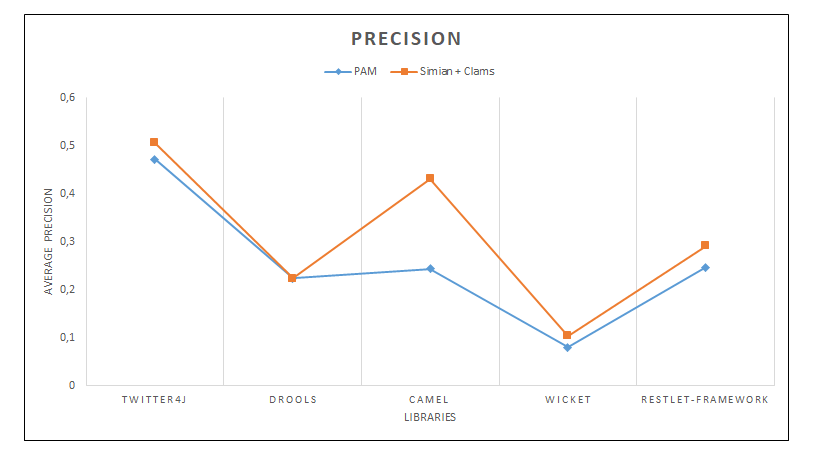
\includegraphics[width=14cm,height=14cm,keepaspectratio]{images/Precision.png}
\centering
  \caption{Precision comparison}
  \label{fig:cmd}
\end{figure}

\begin{figure}[H]
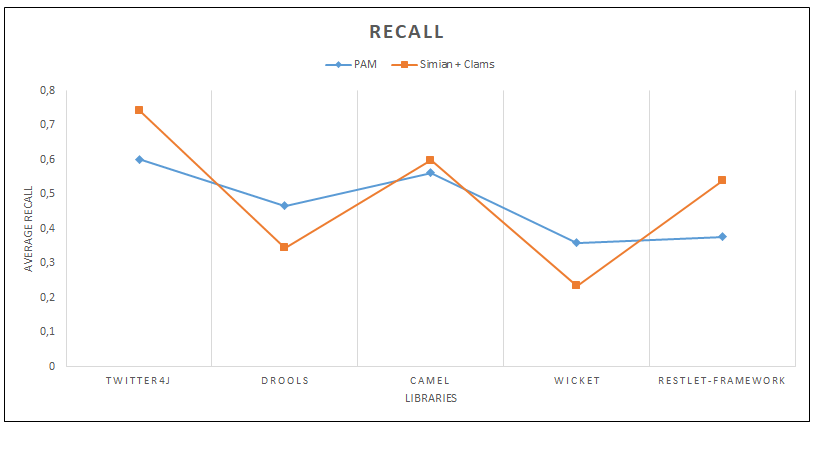
\includegraphics[width=14cm,height=14cm,keepaspectratio]{images/Recall.png}
\centering
\caption{Recall comparison}
\label{fig:cmd}
\end{figure}


\begin{figure}[H]
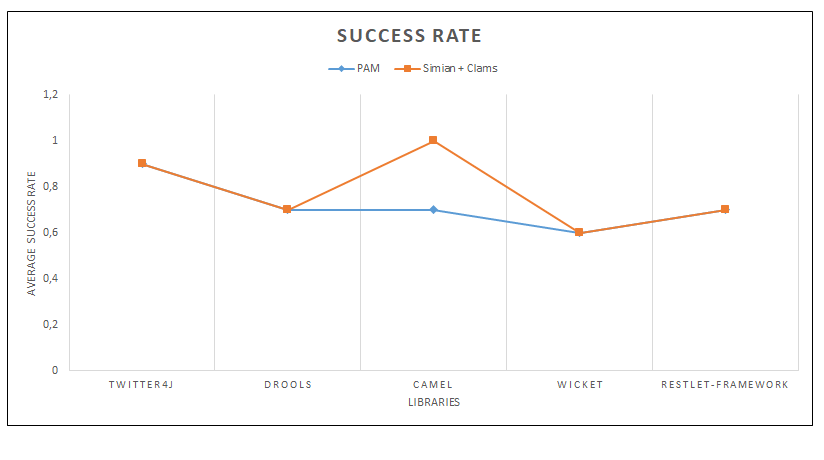
\includegraphics[width=14cm,height=14cm,keepaspectratio]{images/SuccRate.png}
\centering
\caption{Success rate comparison}
\label{fig:cmd}
\end{figure}


\begin{figure}[H]
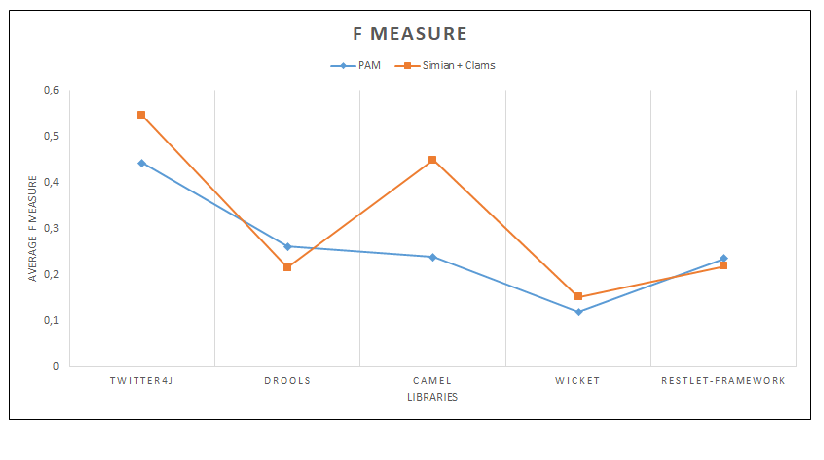
\includegraphics[width=14cm,height=14cm,keepaspectratio]{images/Fmeasure.png}
\centering
\caption{F measure  comparison}
\label{fig:cmd}
\end{figure}


Moreover, we make a time comparison on the computation of the two considered approach, as we pointed out in the \textbf{RQ$_3$}: for PAM, we pick the time needed to produce the list of method invocations starting from a single ARFF file that summarize the context as described before while for our approach, we considered the time needed to produce the recommendations in form of code snippet, considering as context the developer's ground truth (in this case the the ARFF is used by CLAMS to produce the patterns chosen as baseline). The results shows that the time are almost equal,except in the case of wicket library. It happens because PAM relies only on ARFF and, in this case, it contains a huge amount of data. Notice that all the evaluation tasks have been executed on Windows 10 operative system with a Intel core i5-3230M 2.60 GHz processor.

\begin{figure}[H]
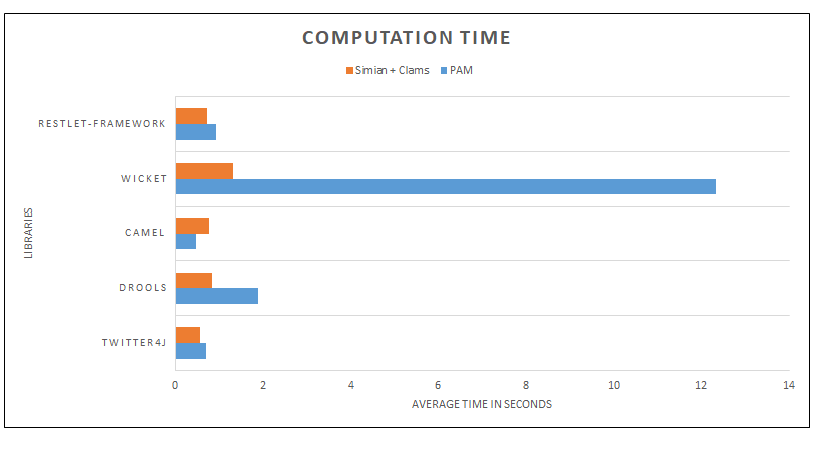
\includegraphics[width=14cm,height=14cm,keepaspectratio]{images/time.png}
\centering
\caption{Time comparison}
\label{fig:cmd}
\end{figure}

The aim of this framework is to give an overall evaluation of accuracy, time, coverage and effectiveness of the API recommendations of the proposed approach. The approach relies on the code cloning activity and, so, the results are not immediately comparable with other existing approaches, as they use other techniques like clustering. For this reason, we need this framework to analyze the results in the proper way and to reduce as much as possible bias that can be led from the different domain and techniques. 
